\documentclass{article}
\usepackage{graphicx} % include figures
\usepackage{xeCJK} % Chinese language support
\usepackage{bm}
\usepackage{amsmath,amsthm,amssymb,amsfonts}
\usepackage{cite}
\usepackage[colorlinks,linkcolor=red,anchorcolor=blue,citecolor=green,CJKbookmarks=true]{hyperref}
\usepackage{indentfirst} % indent before a paragraph, Chinese-style
\usepackage{amsmath}
\usepackage[margin=3.5cm]{geometry}
\usepackage{titlesec}
\usepackage{amsmath}
\usepackage{amssymb}
% \linespread{1.6}
\geometry{left=3.2cm,right=3.2cm,top=3.2cm,bottom=3.2cm}
\usepackage{booktabs}
\usepackage{multirow}
\usepackage{array} % assign height for tables
\usepackage{listings}
\usepackage{xcolor}
\usepackage{ulem}
\usepackage{enumitem}
\usepackage{tikz}
\usepackage{lipsum}
\usepackage{empheq} % enable eq numbering inside a brace
\usepackage{float} % forces figs to appear precisely at the location in code
\usepackage[section]{placeins} % prevents figs appearing after its section

\usepackage{mdframed} % when codes cross pages, this is used to add a frame
\setenumerate[1]{itemsep=0pt,partopsep=0pt,parsep=\parskip,topsep=5pt}
\setitemize[1]{itemsep=0pt,partopsep=0pt,parsep=\parskip,topsep=5pt}
\setdescription{itemsep=0pt,partopsep=0pt,parsep=\parskip,topsep=5pt}
% therom
\makeatletter
\thm@headfont{\sc}
\makeatother
\newtheorem{theorem}{Theorem}

\usepackage{hyperref}% keeps internal links (include table of contents) black
\hypersetup{%
  colorlinks = true,
  linkcolor  = black
}

%%%%%%%%%%%%% MATLAB configuration %%%%%%%%%%%%%
%\usepackage{listings} % used for code highlight
%\lstset{extendedchars=false}%这一条命令可以解决代码跨页时,章节标题,页眉等汉字不显示的问题
%\usepackage[framed,numbered,autolinebreaks]{mcode}
\usepackage[T1]{fontenc}
\usepackage[numbered,framed]{matlab-prettifier}
\usepackage{filecontents}
\let\ph\mlplaceholder % shorter macro
\lstMakeShortInline"
\lstset{
  style              = Matlab-editor,
  basicstyle         = \mlttfamily,
  escapechar         = ",
  mlshowsectionrules = true,
}
%\begin{filecontents*}{/code/LIP_straightline.m}

%%%%%%%%%%%% MATLAB configuration %%%%%%%%%%%%%%

%\setCJKmainfont[BoldFont = 黑体]{宋体}
%\setlength{\parindent}{2em} %设置段首空两格
%如果不要缩进 用\noindent

%%%%%%%%%%%%%%%%%%%%%%%%%%%%%%%%%%%%%%%%%%%%%%%%%%%%%%%%%%%%%%%%%%%%%%%%
%%%%%%%%%%%%%%%%%%%%%%%%%%%%%%%%%%%%%%%%%%%%%%%%%%%%%%%%%%%%%%%%%%%%%%%%
%%%%%%%%%%%%%%%%%%%%%%%%%%%%%%%%%%%%%%%%%%%%%%%%%%%%%%%%%%%%%%%%%%%%%%%%
%%%%%%%%%%%%%%%%%%%%          Article             %%%%%%%%%%%%%%%%%%%%%%
%%%%%%%%%%%%%%%%%%%%%%%%%%%%%%%%%%%%%%%%%%%%%%%%%%%%%%%%%%%%%%%%%%%%%%%%
%%%%%%%%%%%%%%%%%%%%%%%%%%%%%%%%%%%%%%%%%%%%%%%%%%%%%%%%%%%%%%%%%%%%%%%%
%%%%%%%%%%%%%%%%%%%%%%%%%%%%%%%%%%%%%%%%%%%%%%%%%%%%%%%%%%%%%%%%%%%%%%%%
\title{ME106 Project1 Report}
\author{\large Rui\hspace{0.5cm}Wang \\ 3033461836}
\date{}
\begin{document}
\maketitle
\vspace{4cm}
\tableofcontents
\clearpage
\section{Part 1: Streamlines}

  \subsection{Problem Statement}
  The problem consists of two parts:
  \begin{itemize}
    \item Given an array of velocity field, plot it with MATLAB \texttt{quiver()} function.
    \item Draw ten streamlines on the plot.
  \end{itemize}

  \subsection{Solution}
  The array is given as a $63 \times 63$ matrix, however, we do not want to hard code it as we wish to apply this algorithm to any dimensions of matrices as well. Plotting the velocity field is straight-forward, and streamlines are obtained by moving along the velocity field with a constant time('snapshot').
  
  \subsection{Code and Plot for Velocity Field}
  First, we plot the velocity field with \texttt{quiver()}. Note that the matrix must be scaled to $[0, 1]$ before plot, so we make use of \texttt{meshgrid()}.
  \lstinputlisting[style=Matlab-editor, caption = {Commands to plot a velocity field.}]{code/quiverPlot.m}
  Figure \ref{fig:vel} is the plot for the velocity field.
  \begin{figure}[H]
    \centering
    \noindent\makebox[\textwidth][c] 
    {
    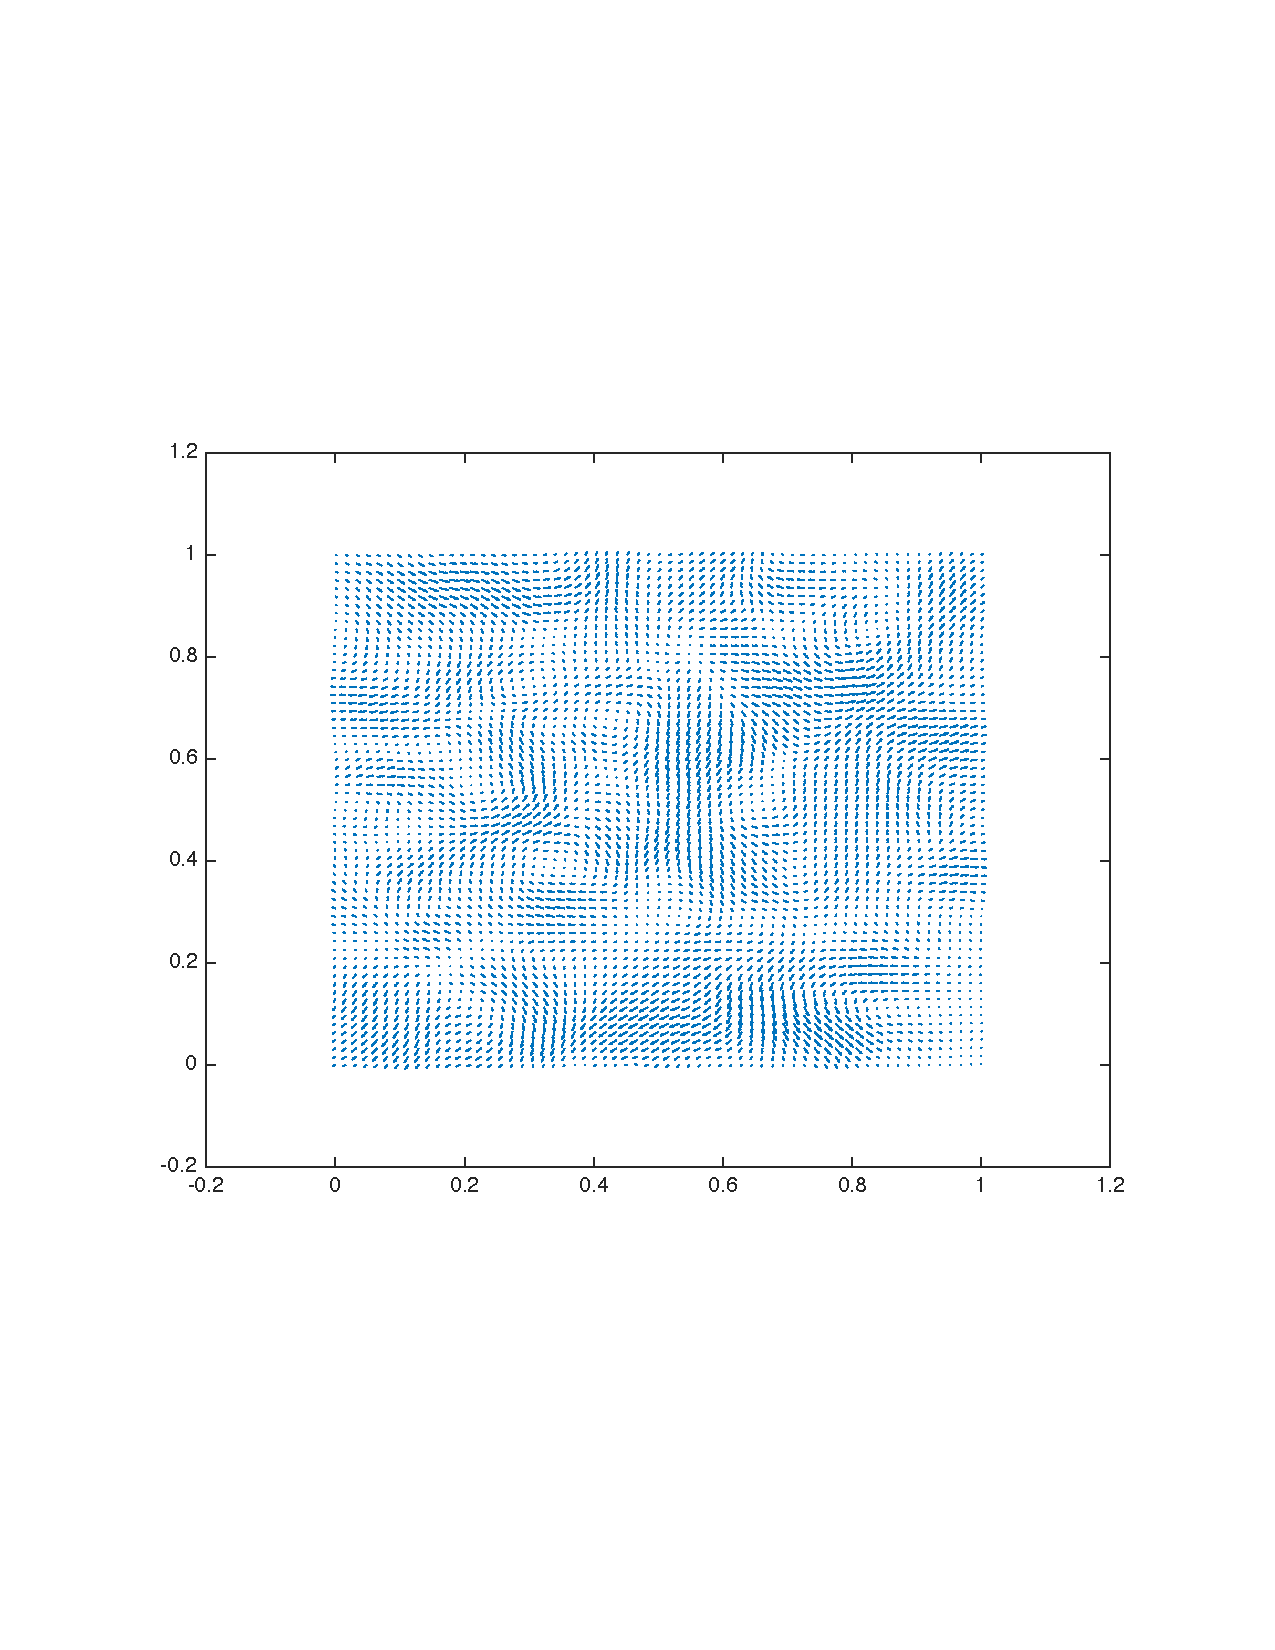
\includegraphics[width=0.5\paperwidth]{images/velocity.pdf}
    }
    \caption{The original velocity field.} \label{fig:vel}
  \end{figure}
  
  \subsection{Code and Plot for Streamline}
  Below is the function to plot a streamline. \texttt{xcoord} and \texttt{ycoord} are references for $x$ and $y$ axis, and can either be a column or row vector. The entire area is presumed to be a rectangle. \texttt{x0} and \texttt{y0} are column vectors, namely the $x$, $y$ axis of a list of starting point of the streamlines to be plotted.
  \lstinputlisting[style=Matlab-editor, caption = {streamlinePlotter.m}]{code/streamlinePlotter.m}
  We then obtain our streamline with the following commands:(using \texttt{ginput()} to obtain ten appropriate starting points on Figure \ref{fig:vel}, so we keep the previous figure open). With the following commands, we can plot our streamline:
  \lstinputlisting[style=Matlab-editor, caption = {Plot the streamline with my function}]{code/stream.m}
  The basic idea is to "walk" out a streamline. As for a streamline, we have
  $$\frac{dx}{u} = \frac{dy}{v} = ds$$ thus we obtain $$dx = uds, dy = vds$$ $dx$ and $dy$ are the distances of our each step.
  \begin{figure}[H]
    \centering
    \noindent\makebox[\textwidth][c] 
    {
    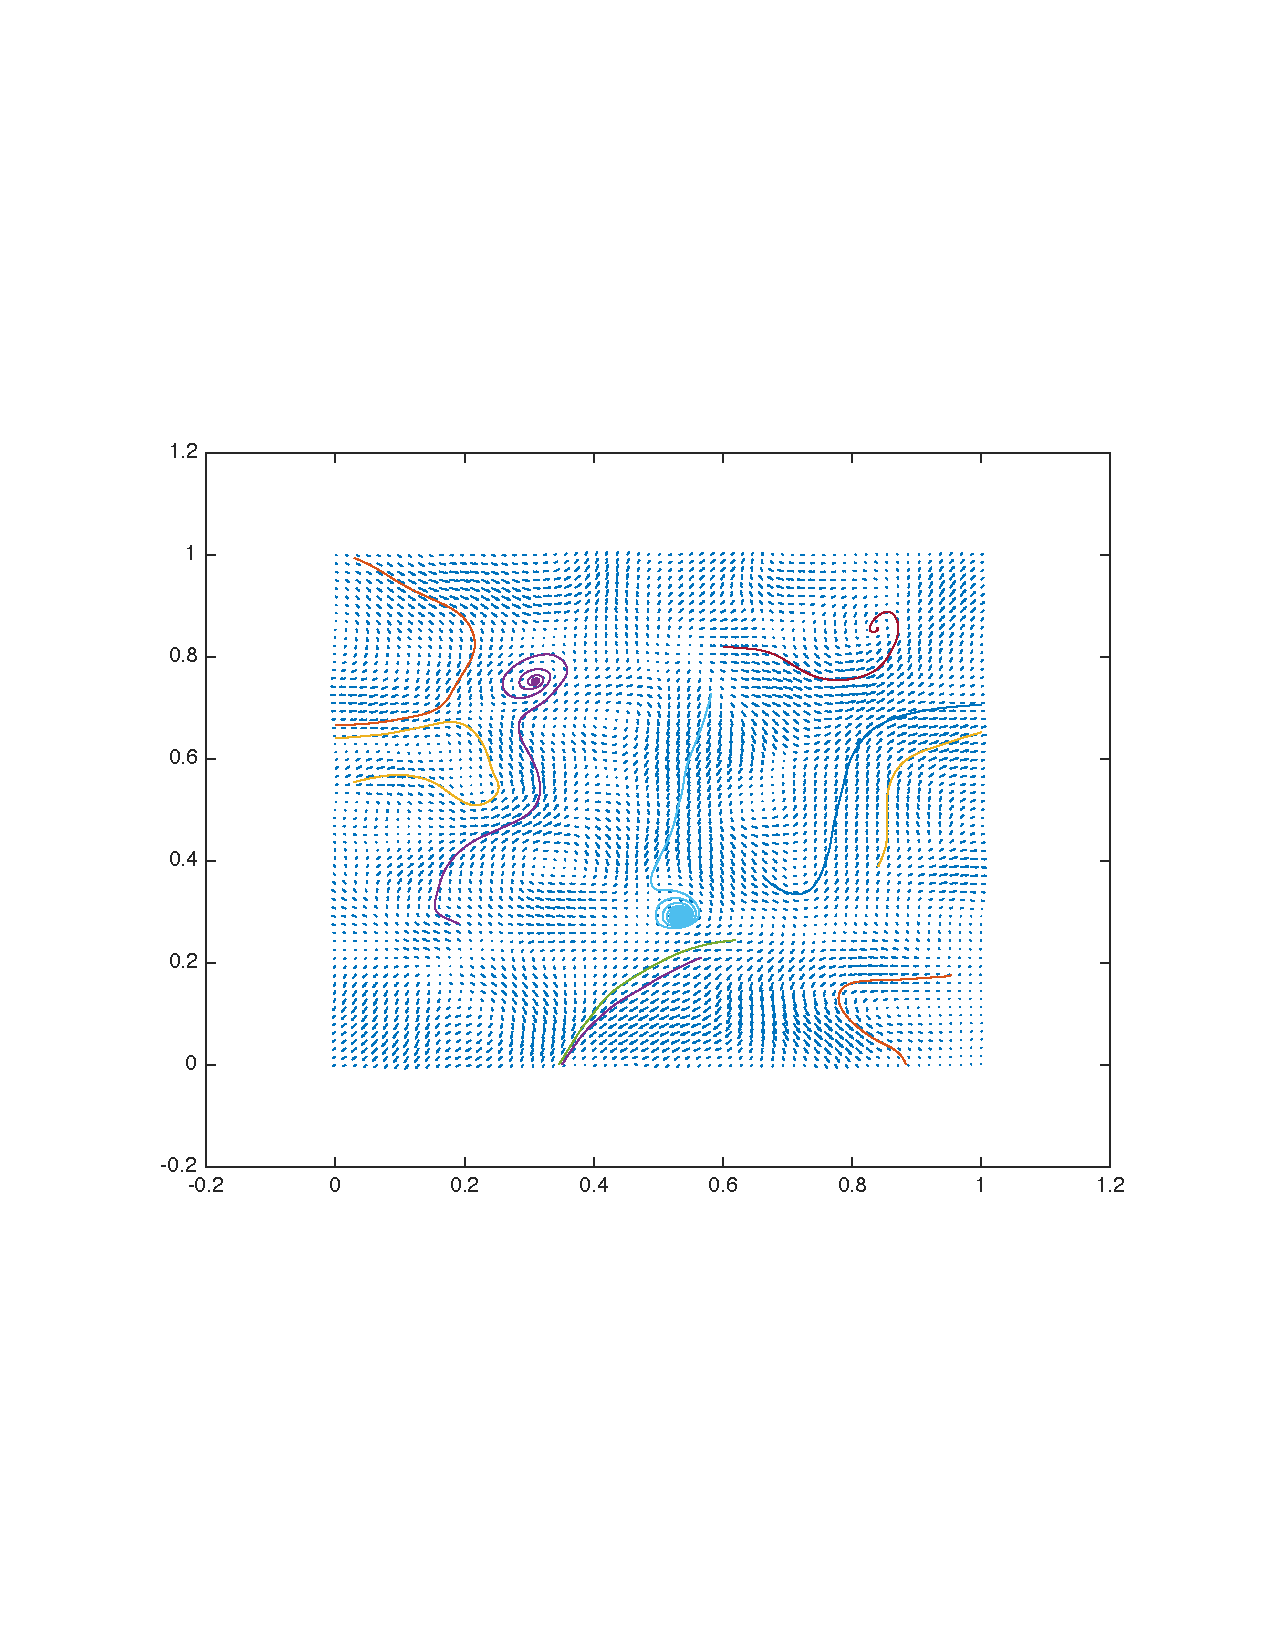
\includegraphics[width=0.5\paperwidth]{images/streamlineOnVel.pdf}
    }
    \caption{Streamlines plotted by my function.} \label{fig:streamline}
  \end{figure}
  We can compare it with MATLAB's \texttt{streamline()} function, the result of which is on Figure \ref{fig:standardStreamline}.
  \begin{figure}
    \centering
    \noindent\makebox[\textwidth][c] 
    {
    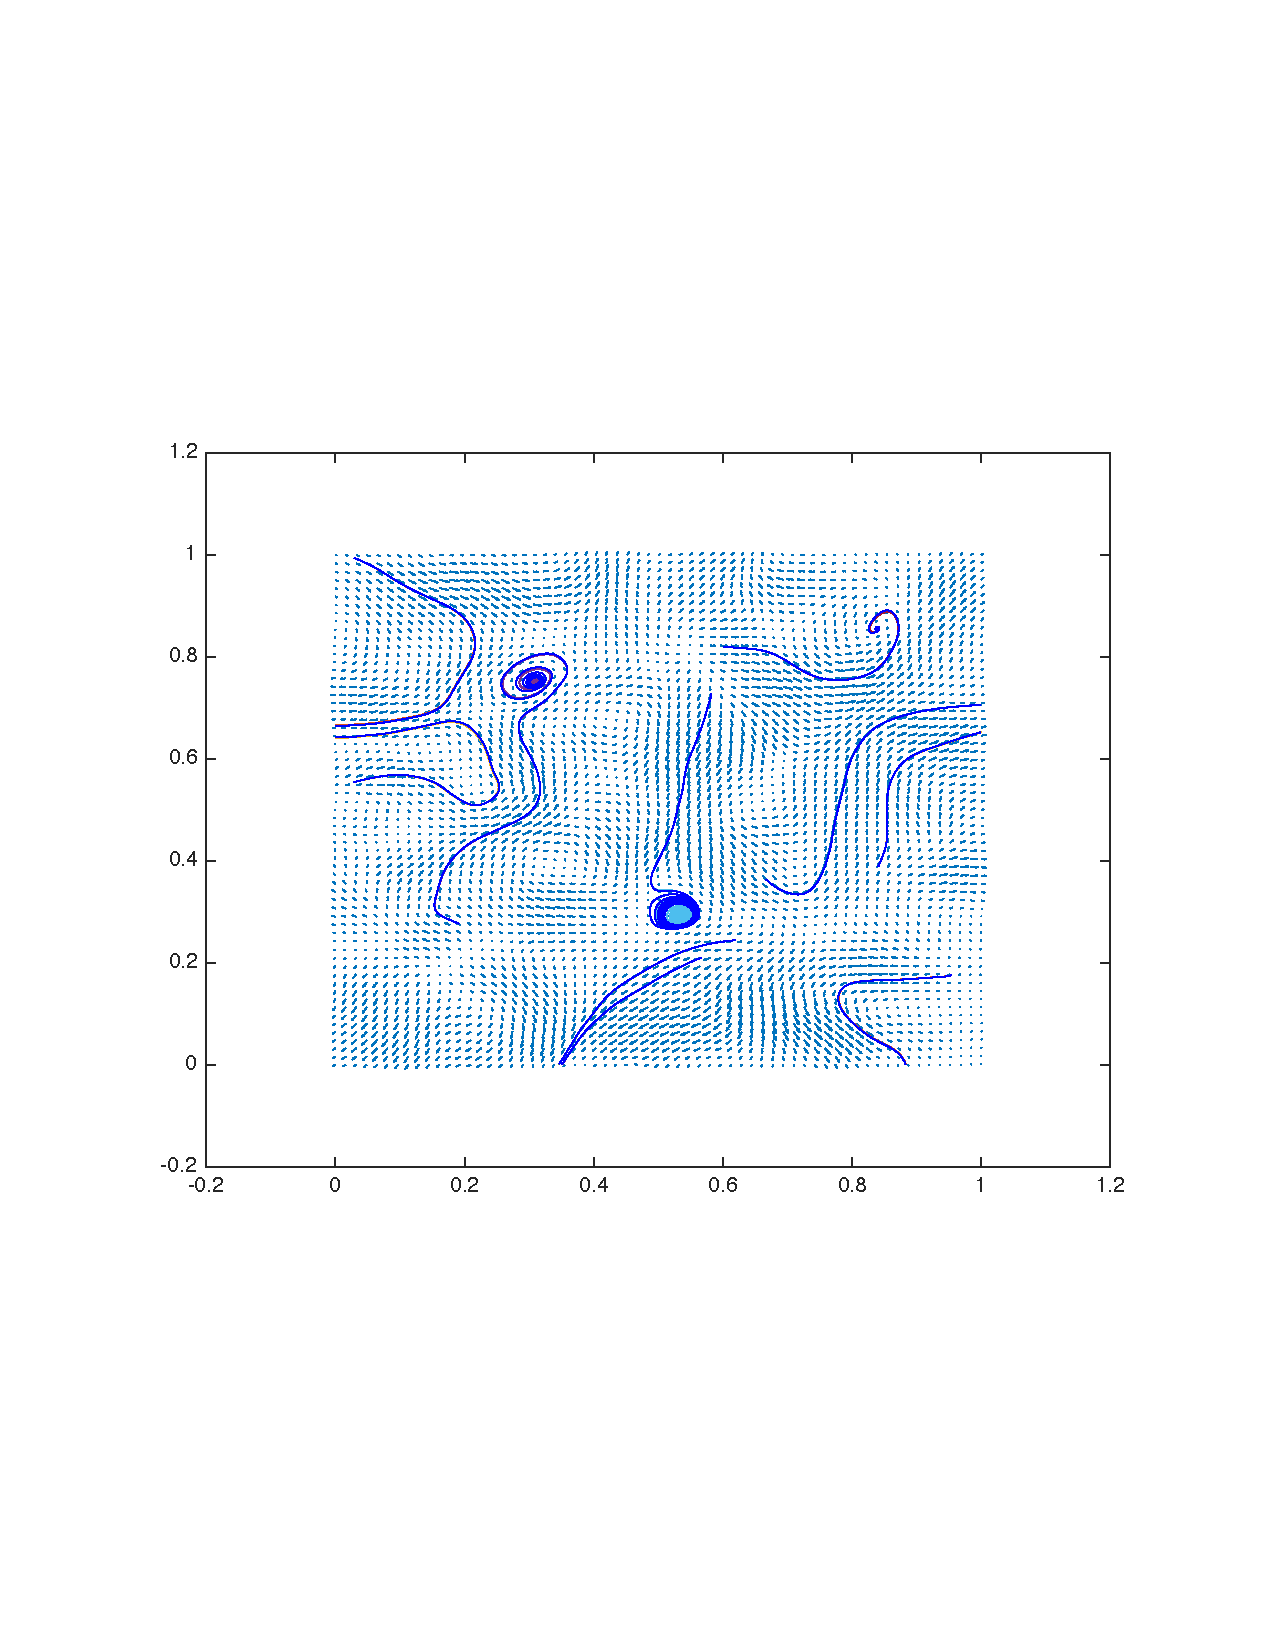
\includegraphics[width=0.5\paperwidth]{images/standardStreamline.pdf}
    }
    \caption{Streamlines plotted by MATLAB.} \label{fig:standardStreamline}
  \end{figure}
  We can observe that the curves of two methods coincide, justifying my implementation. Note that on Figure \ref{fig:standardStreamline}, the new curve is directly plotted upon the previous one. The dark blue lines are plotted by MATLAB's \texttt{streamline()}. We can see that there is a little difference(especially on the vortex in the middle), this is because we are using a fixed step of $ds = 0.001$, which can yield inaccurate estimation at certain locations where the curvature is very large.
  
  \section{Part 2: Flow around a Moving Cylinder}
  \subsection{Problem Satatement}
  The flow velocity field around a cylinder is given. Since $a = 1$ and $U = 1$ throughout the problem, we directly plug in these two constants and get the following expression:
  $$u = \frac{(x+t)^2 - y^2}{((x+t)^2+y^2)^2}$$
  $$v = \frac{2(x+t)y}{((x+t)^2+y^2)^2}$$
  We are required to
  \begin{itemize}
    \item plot the velocity field using \texttt{contourf()} when $t = 0$.
    \item Plot 8 streamlines with given starting point.
    \item Plot a pathline.
  \end{itemize}
  
  \subsection{Solution Code and Result for Velocity Field}
  With a first trial, we will see that the velocity goes to infinity very quickly at around the origin. This makes the contour extremely ugly, so we sort to draw the contour not based on a uniform distance in velocity, but on a gradual gradient.\par
  One thing to note is that we need to enlarge each step from $0.001$ to maybe $0.01$ in this implementation to allow for a faster calculation. Otherwise we will have to wait for a very long time before the plot can be finished.\par
  Below is the code for the first two requirements of this problem.
  \lstinputlisting[style=Matlab-editor, caption = {Velocity contour plotting and streamline at given points.}]{code/part2.m}
  This yields 
  \begin{figure}[H]
    \centering
    \noindent\makebox[\textwidth][c] 
    {
    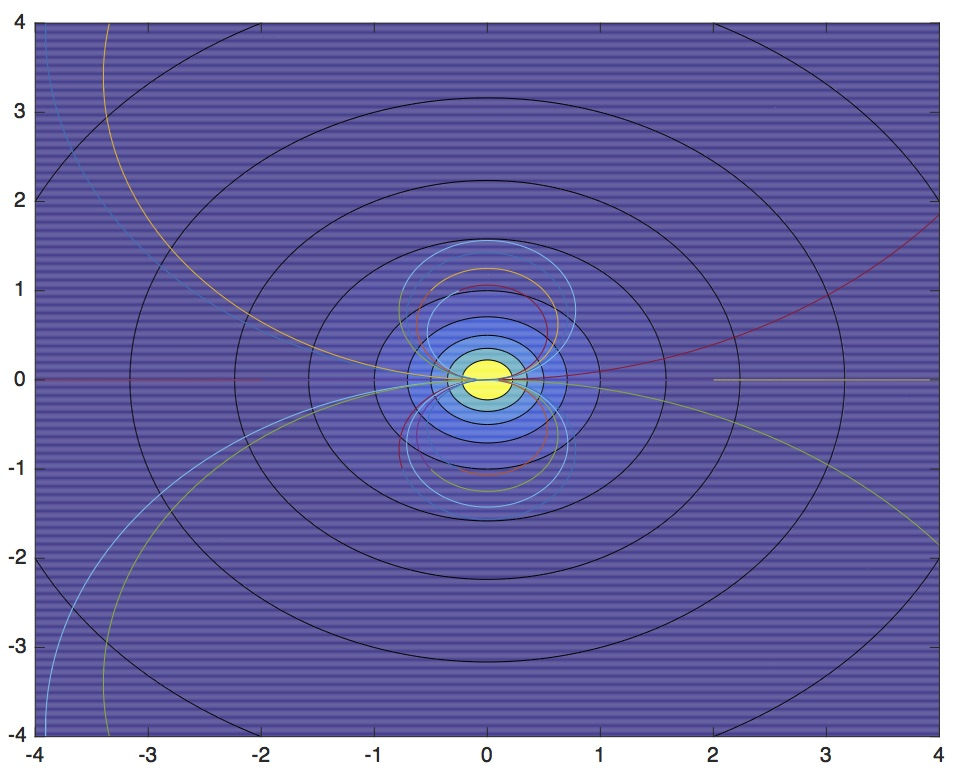
\includegraphics[width=0.5\paperwidth]{images/part2-2.pdf}
    }
    \caption{Velocity Contour and Streamlines} \label{fig:part2}
  \end{figure}
  In Figure \ref{fig:part2}, black lines indicate the contour, while colored lines are those streamlines.\par
  
  \subsection{Code and Result for Pathline}
  For the pathline problem, we use basically the same method as problem Part 1, except for that we include time $t$ as a variable in this numerical simulation. One problem is that the velocity of the bug is expressed as $u_r$ and $u_{\theta}$, while in reality if we want to calculate the next position for the bug we need the $x$, $y$ coordinates. So we will need to convert from polar to cartesian.
  
  $$u_x = u_rcos\theta - u_{\theta}sin\theta$$
  $$u_y = u_rsin\theta + u_{\theta}cos\theta$$
  
  Hereafter we can update the bug's position by $x_t = x_{t-dt} + u_x dt$ and $y_t = y_{t-dt} + u_y dt$.
  
  \lstinputlisting[style=Matlab-editor, caption = {}]{code/pathlinePlotter.m}
  The result of the pathline is a bit boring, as shown in Figure \ref{fig:pathline}.
  \begin{figure}[H]
    \centering
    \noindent\makebox[\textwidth][c] 
    {
    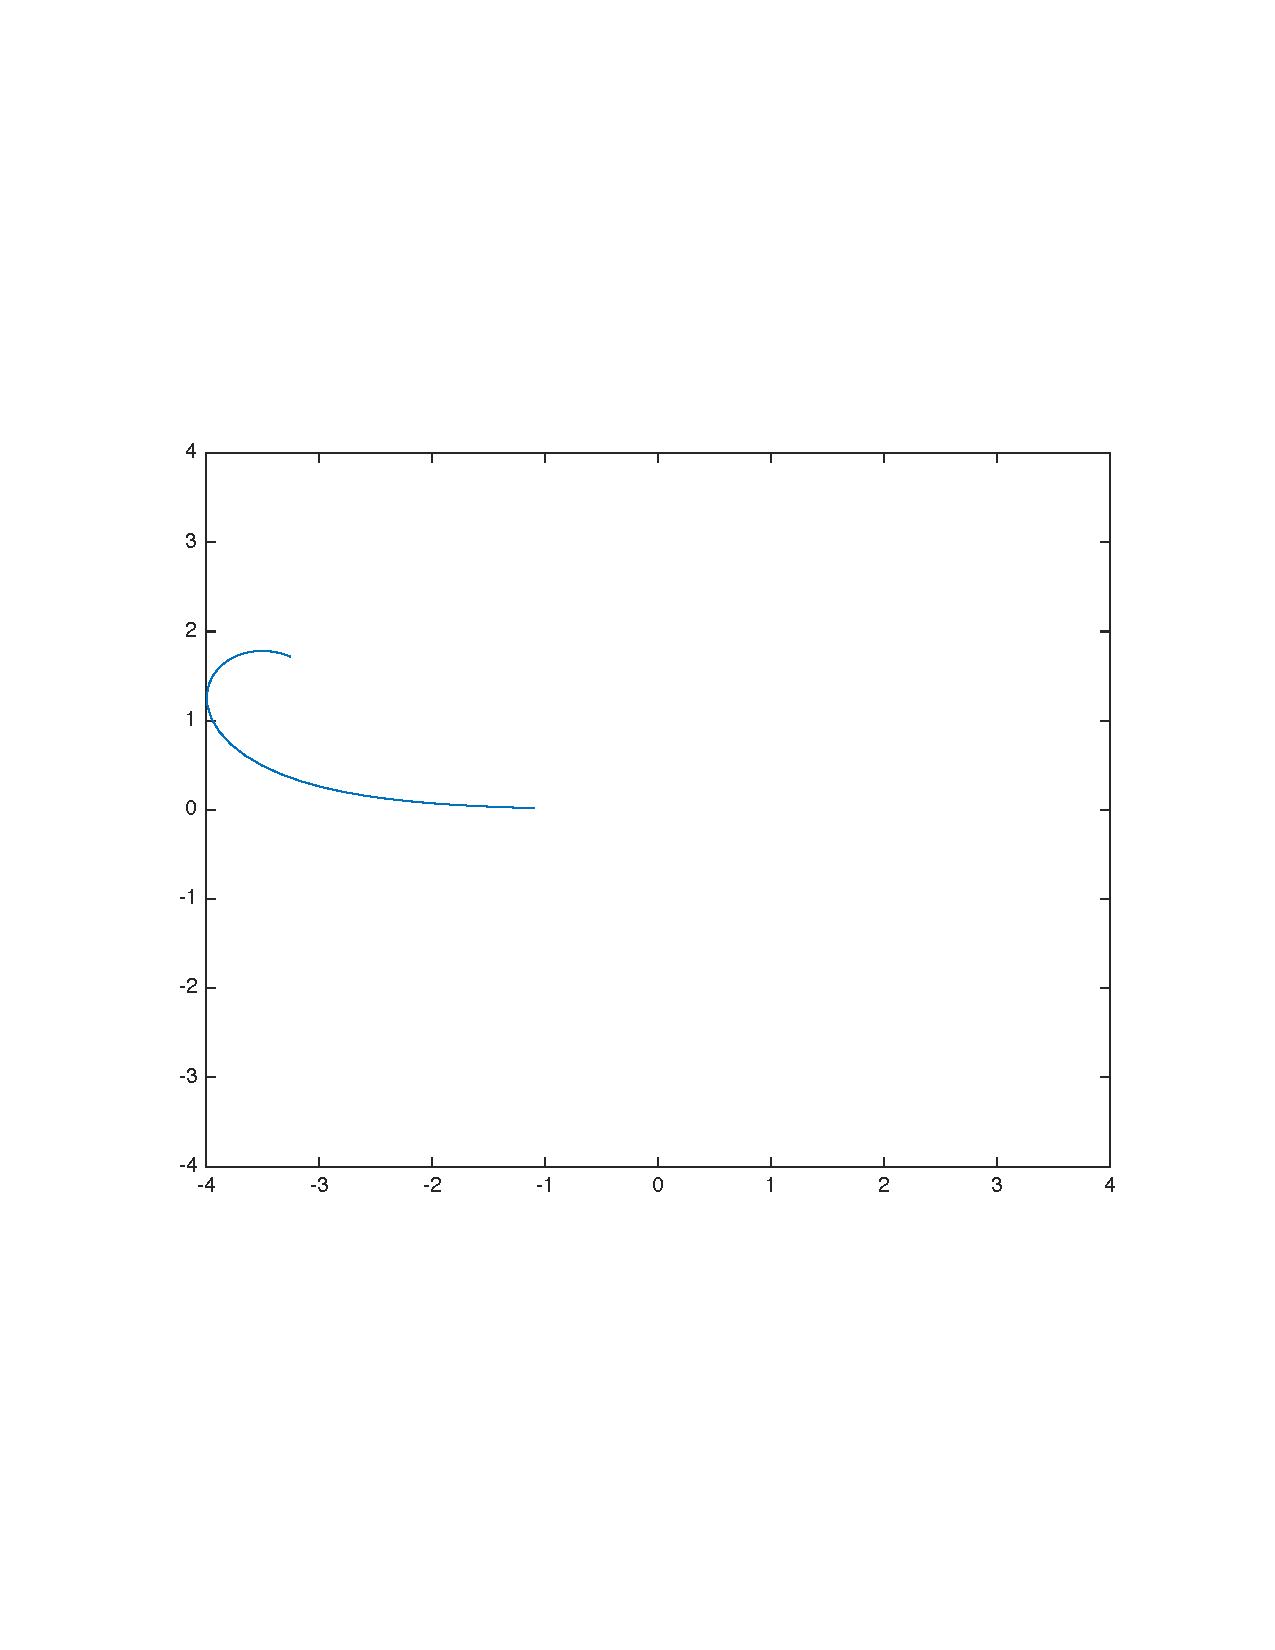
\includegraphics[width=0.4\paperwidth]{images/pathline.pdf}
    }
    \caption{Pathline of a Bug} \label{fig:pathline}
  \end{figure}
  However, the size of the step may affect the plotting result, so the pathline is not rigorous.
%  However, the size of the step may significantly affect the plotting result. Reducing the time step to $0.01$, for example, yields the following curve, which is more accurate:
%  \begin{figure}[H]
%    \centering
%    \noindent\makebox[\textwidth][c] 
%    {
%    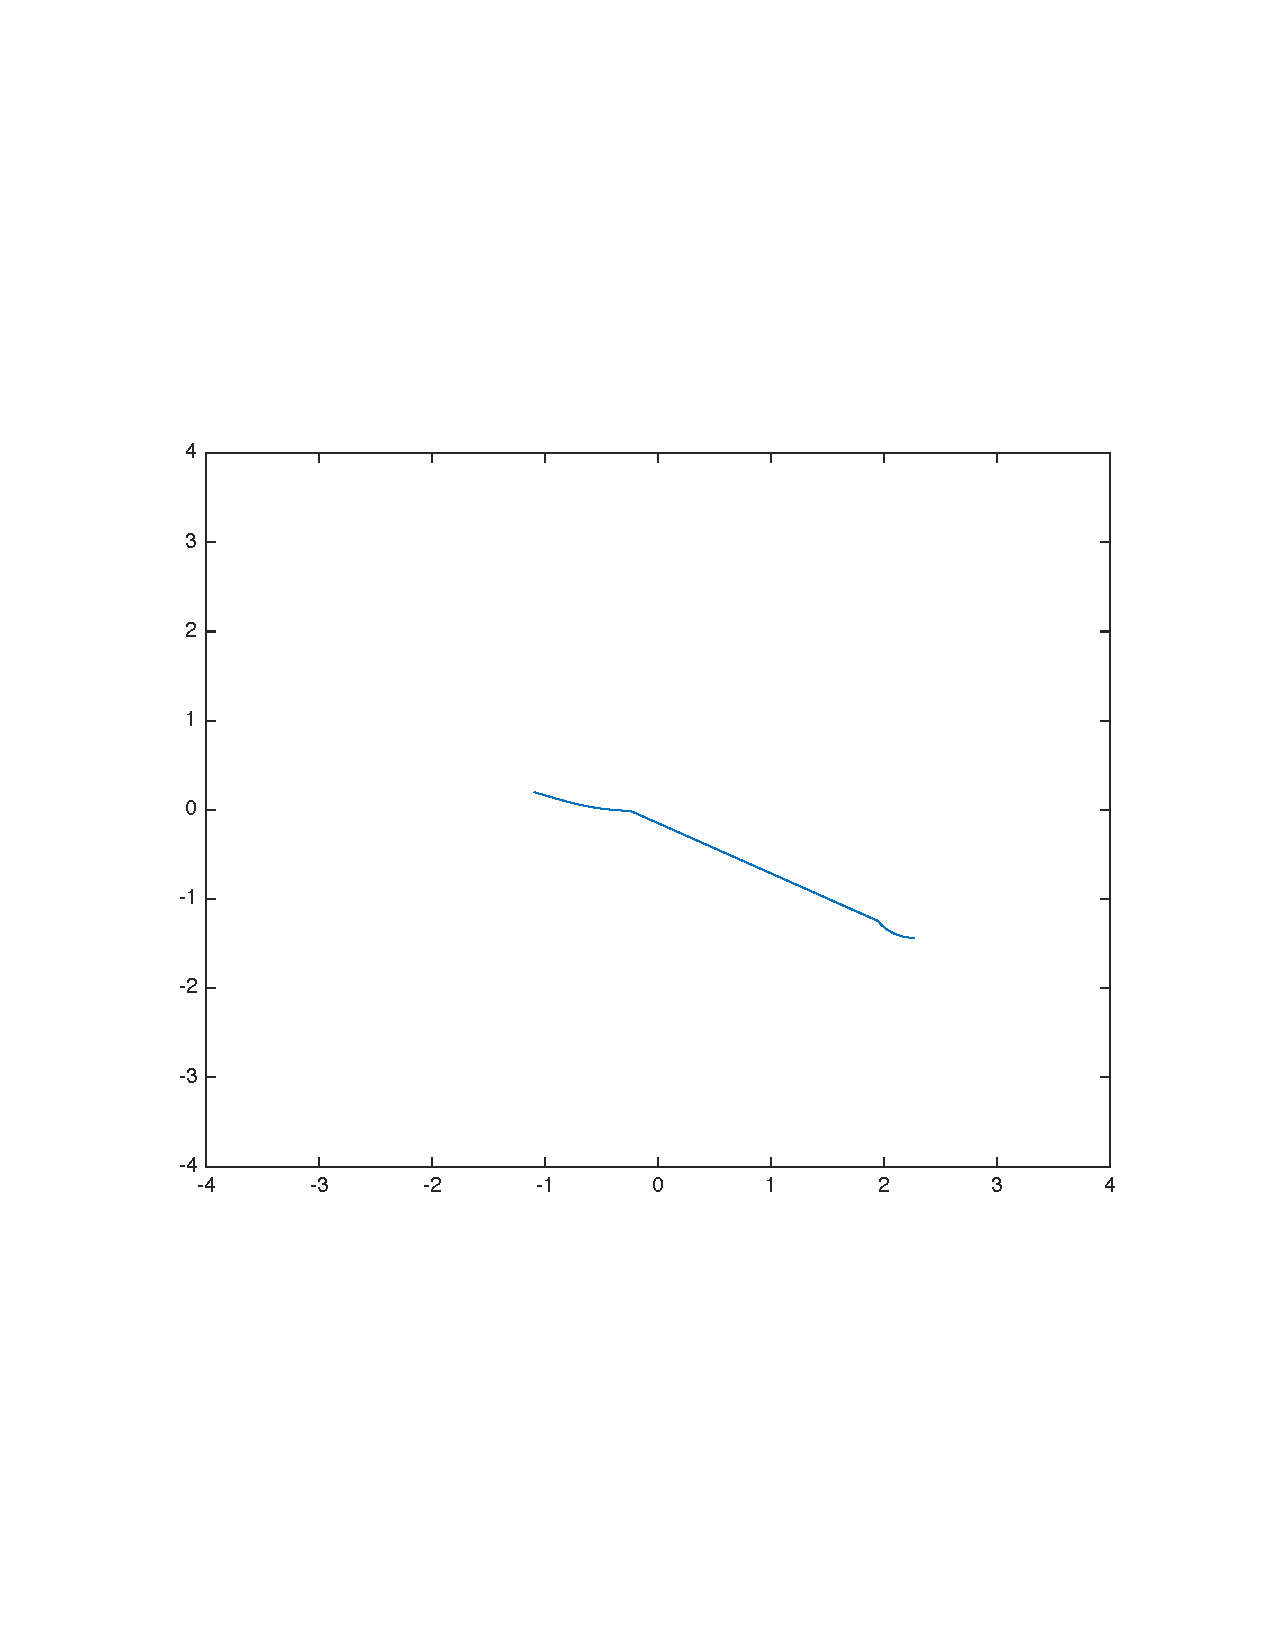
\includegraphics[width=0.5\paperwidth]{images/reduced.pdf}
%    }
%    \caption{Pathline with a Reduced Time Step} \label{fig:reduced}
%  \end{figure}

  
\clearpage % print all figures above before new a page
%\appendix
%Appendix:
%
%\lstinputlisting[style=Matlab-editor, caption = {RLCdynamics.m}]{code/RLCdynamics.m}
    %%%%%%%%%%%%%%%
    %%%%%%%%%%%%%%%
    %  CODE HERE  %
    %%%%%%%%%%%%%%%
    %%%%%%%%%%%%%%%
%\lstinputlisting[style=Matlab-editor]{code/RLCdynamics.m}

\end{document}